\documentclass[a4paper]{article}
\usepackage[UTF8]{ctex}
\usepackage{geometry}
\usepackage{graphicx}
\usepackage{url}
\usepackage{multirow}
\usepackage{array}
\usepackage{booktabs}
\usepackage{url}
\usepackage{enumitem}
\usepackage{graphicx}
\usepackage{float}
\usepackage{amssymb}
\usepackage{amsmath}
\usepackage{subfig}
\usepackage{longtable}
\usepackage{pifont}
\usepackage{color}

\allowdisplaybreaks

\geometry{a4paper, scale=0.78}

% \begin{figure}[H]
%     \centering
%     \includegraphics[width=.55\textwidth]{E.png}
%     \caption{矩阵与列向量的乘法}
%     \label{fig:my_label_1}
% \end{figure}

% \left\{
% \begin{array}{ll}
%       x+2x+z=2 & \\
%       3x+8y+z=12 & \\
%       4y+z=2
% \end{array}
% \right.

% \begin{enumerate}[itemindent = 1em, itemsep = 0.4pt, parsep=0.5pt, topsep = 0.5pt]

% \end{enumerate}

%\stackrel{a}{\longrightarrow}

%\underbrace{}_{} %下括号

%\tableofcontents %目录,并且目录页不记录页码
% \tableofcontents
% \newpage
% \setcounter{page}{1} %new page
% \clearpage

\title{Particle Filter}
\author{Chen Gong}
\date{09 February 2020}

\begin{document}
% \textrm{Roman Family}
\maketitle
%\pagestyle{empty}
\tableofcontents
\newpage
%\pagestyle{fancy}
\setcounter{page}{1} %new page
\clearpage

\section{背景介绍}
Dynamic Model是在概率图模型中加入了时序的因素,所以样本之间不再是独立同分布(i.i.d)的,而是有依赖关系的。而Dynamic Model的一个主要特点是,混合模型。因为,我们看到的都是观测变量序列,而每一个观测变量都对应着一个隐变量,隐变量也被称之为系统变量(System Variable),所以有时我们也将Dynamic Model称之为State Space Model。

而Dynamic Model我们可以从两个假设,两个方程,三个问题的角度去分析。

\subsection{两个假设}
这是有关Dynamic Model的两个假设,也是我们研究这个模型的前提条件。这两个假设可以大大的帮助我们简化模型:

1.\textbf{ 齐次Markov假设(无后向性):}未来与过去无关,只依赖与当前的状态。数学公式描述也就是。
\begin{equation}
    P(i_{t+1}|i_{t},i_{t-1},\cdots,i_1,o_t,\cdots,o_1) = P(i_{t+1}|i_t)
\end{equation}

2. \textbf{观测独立假设:}当前时刻的观测变量只依赖于当前时刻的隐变量。
\begin{equation}
    P(o_{t}|i_{t},i_{t-1},\cdots,i_1,o_t,\cdots,o_1) = P(o_{t}|i_t)
\end{equation}

\subsection{两个方程}
这两个方程分别描述的是,隐变量状态与状态之间的转移概率,由当前时刻隐变量推出当前时刻观测变量的概率,符合化描述如下所示:
\begin{equation}
    \left\{
        \begin{array}{ll}
            z_t = g(z_{t-1},\mu,\xi) & \\
            x_t = h(z_{t},\mu,\delta) & \\
        \end{array}
    \right.
\end{equation}
经过类比,我们就可以很简单的发现,$g(\cdot)$函数就是HMM中的状态转移矩阵$A$,$h(\cdot)$函数就是HMM中的发射转移矩阵$B$。

\subsection{三大类问题}
在Dynamic Model中,我们主要可以分为三大类问题。
\subsubsection{隐马尔可夫模型(Hidden Markov Model)}
这个在之前的章节中,我们已经有了详细的讲解。主要特点就是,隐状态$z$之间是离散的,而观测变量$s$之间并没有限制。在Hidden Markov Model中,主要关注的是Decoding问题,也就是在已知观测序列的情况下,最大化可能的隐状态。

\subsubsection{线性动态系统(Linear Dynamic System)}
线性动态系通常也被我们称为线性高斯系统,而线性高斯系统这个名字更加形象,而线性和高斯的来源主要如下所示:
\begin{equation}
    \left\{
        \begin{array}{ll}
            z_t = A\cdot z_{t-1}+B+\epsilon & \epsilon \sim \mathcal{N}(0,Q) \\
            x_t = C\cdot z_{t}+D+\delta & \delta \sim \mathcal{N}(0,R)\\
        \end{array}
    \right.
\end{equation}
也就是式(3)中的两个函数将符合线性和噪声符合Gaussian Distribution的原则。而Dynamic Model中重点关注的就是Filter问题,Filter问题就是求解$P(z_t|x_1,x_2,\cdots,x_t)$,在已知观测序列的情况下,求解当前时刻的隐变量的状态。

\subsubsection{Filter问题的求解}
我们的求解目标是$P(z_t|x_1,x_2,\cdots,x_t)$。

Step 1. Prediction:这个过程我们可以理解成给$z_t$一个先验,
\begin{equation}
    P(z_t|x_1,x_2,\cdots,x_{t-1}) = \int_{z_{t-1}} P(z_t|z_{t-1}) P(z_{t-1}|x_1,x_2,\cdots,x_{t-1}) dz_{t-1}
\end{equation}

Step 2. Update:这个过程我们可以理解成给$z_t$在已知$x_t$之后的后验,
\begin{equation}
    P(z_t|x_1,x_2,\cdots,x_t) \propto P(x_t|z_t)\cdot P(z_t|x_1,x_2,\cdots,x_{t-1})
\end{equation}

\subsubsection{Preiction的证明}
\begin{equation}
    \begin{split}
        P(z_t|x_1,x_2,\cdots,x_{t-1}) 
        = & \int_{z_{t-1}} P(z_t,z_{t-1}|x_1,x_2,\cdots,x_{t-1}) dz_{t-1} \\
        = & \int_{z_{t-1}} P(z_t|z_{t-1},x_1,x_2,\cdots,x_{t-1}) P(z_{t-1}|x_1,x_2,\cdots,x_{t-1}) dz_{t-1} \\
    \end{split}
\end{equation}

根据Markov齐次假设,$P(z_t|z_{t-1},x_1,x_2,\cdots,x_{t-1})=P(z_t|z_{t-1})$,$P(z_{t-1}|x_1,x_2,\cdots,x_{t-1})$就是$t-1$时刻的data。替换一下就可以得到公式(5)。

\subsubsection{Update的证明}
首先,我们提一下,$P(x_1,x_2,\cdots,x_t)$这种,只和观察数据有关的概率分布都是可以计算出来的,我们都用不同的常数来表示。:
\begin{equation}
    \begin{split}
        P(z_t|x_1,x_2,\cdots,x_t) 
        = & \frac{P(z_t,x_1,x_2,\cdots,x_t)}{P(x_1,x_2,\cdots,x_t)}  \\
        = & \frac{1}{C} P(z_t,x_1,x_2,\cdots,x_t) \\
        = & \frac{1}{C} \underbrace{P(x_t|z_t,x_1,x_2,\cdots,x_{t-1})}_{P(x_t|z_t)}P(z_t,x_1,x_2,\cdots,x_{t-1}) \\
        = & \frac{1}{C} P(x_t|z_t)P(z_t|x_1,x_2,\cdots,x_{t-1})\underbrace{P(x_1,x_2,\cdots,x_{t-1})}_{const\ D} \\
        = & \frac{D}{C}P(x_t|z_t)P(z_t|x_1,x_2,\cdots,x_{t-1})
    \end{split}
\end{equation}
而$P(x_t|z_t)$就是发射矩阵,$P(z_t|x_1,x_2,\cdots,x_{t-1})$就是$t-1$时刻的Prediction。

由于多维Gaussian Distribution非常强大的自共轭性,所以条件概率,边缘概率,联合概率这些都是Gaussian Distribution的,所以可以将高维的高斯分布进行拆解成多个低维的来进行求解就会简单一点。而Linear Dynamic System也被称为Kalman Filter。

\subsection{非线性动态系统(Non-Linear Dynamic System)}
Non-Linear Dynamic System和Linear Dynamic System区别是,相邻两个隐变量状态$z_t$和$z_{t-1}$之间的关系是任意的,而且,Noise也是Gaussian的。所以,无法使用Kalman Filter一样的方法得到解析解。所以,只能采用Monte-Carlo Sampling一样的采样方法来得出近似解。

Non-Linear没有那么好的特征,求不出,只能采样。在贝叶斯框架的Inference主要要求解的是一个后验分布$P(Z|X)$。而这个分布主要是用来求解期望,$\mathbb{E}_{z|x}[f(x)] = \int f(z)p(z|x)dx$。如果,我们可以采取$N$个样本,$z^{(i)}\sim P(Z|X),\{ z^{(1)},z^{(2)},\cdots,z^{(N)} \}$。那么,我们就可以通过$\frac{1}{N}\sum_{i=1}^N f(z^{(i)})$来求解。这就是最简单的Monte-Carlo Sampling的方法。

\section{重要性采样(Importance Sampling)}
重要性采样并不是直接对概率分布进行采样,而是对提议(Proposal)分布进行采样。也就是:
\begin{equation}
    \begin{split}
        \mathbb{E}_{p(z)}[f(z)] = \int p(z)f(z)dz 
        = & \int \frac{p(z)}{q(z)} q(z)f(z)dz \\
        = & \int f(z)\frac{p(z)}{q(z)} q(z)dz \\
        \approx & \frac{1}{N} \sum_{i=1}^N f(z_i) \frac{p(z_i)}{q(z_i)}\ (z_i \sim q(z),\ i = 1,2,\cdots,N)
    \end{split}
\end{equation}

而这里的$\frac{p(z_i)}{q(z_i)}$也就是Weight,用来平衡不同的概率密度值之间的差距。同样重要性采样也可能会出现一些问题,就是两个分布之间的差距太大了话,总是采样采不到重要的样本,采的可能都是实际分布概率值小的部分。也就是采样效率不均匀的问题。

{\color{red} 之后为了方便描述,我们用$x_{1:t} = x_1,x_2,\cdots,x_t$。}

如果是在Filtering的问题中,目标是求解$P(z_t|x_{1:t})$,权值为:
\begin{equation}
    w^{(i)}_t = \frac{P(z_t^{(i)}|x_{1:t})}{Q(z_t^{(i)}|x_{1:t})}
\end{equation}
而在每一个时刻,都有$N$个样本点:
\begin{equation}
    \begin{split}
        & t=1:\ w^{(i)}_1,\ i=1,2,\cdots,N \sim w^{(1)}_1,w^{(2)}_1,\cdots,w^{(N)}_1 \\
        & t=2:\ w^{(i)}_2,\ i=1,2,\cdots,N \sim w^{(1)}_2,w^{(2)}_2,\cdots,w^{(N)}_2 \\
        & \cdots\cdots \\
        & t=T:\ w^{(i)}_T,\ i=1,2,\cdots,N \sim w^{(1)}_T,w^{(2)}_T,\cdots,w^{(N)}_T \\
    \end{split}
\end{equation}
而实际上$P(z_t^{(i)}|x_{1:t})$的求解非常的复杂,而这样的迭代式求解,实际上复杂度非常的高。我们计算起来非常的复杂。我们想在$w^{(i)}_T$和$w^{(i)}_{T-1}$之间寻找一个递推关系式来大大的简化计算。然后就引出了下面的Sequential Importance Sampling (SIS)算法。

\section{顺序重要性采样(Sequential Importance Sampling)}
这个算法中的主要思想就是,找到$w^{(i)}_T$和$w^{(i)}_{T-1}$之间的一个递推关系式来简化计算。

在这个算法的开始,做出了一个我觉得有点神奇的铺垫。那就是将求解的重点做了一个转变:
\begin{equation}
    P(z_t|x_{1:t}) \longrightarrow P(z_{1:t}|x_{1:t}) 
\end{equation}
实际上$P(z_t|x_{1:t})$是$P(z_{1:t}|x_{1:t})$的一个边缘概率分布,而老师讲了一个很自然我们可以直接丢弃$z_{1:t-1}$,从而使得$P(z_t|x_{1:t})$和$P(z_{1:t}|x_{1:t})$等价处理。本人水平有限,所以实在没有想清楚这到底是怎样一个自然法。所以,我理解的是,在$x_{1:t}$都知道的情况下,$P(z_{1:t}|x_{1:t})$的边缘概率求起来比较方便。大家有什么好的想法,欢迎留言讨论。

而$P(z_{1:t}|x_{1:t})$对应的权重$w_t^{(i)}$为:
\begin{equation}
    w_t^{(i)} \propto \frac{P(z_{1:t}^{(i)}|x_{1:t})}{Q(z_{1:t}^{(i)}|x_{1:t})}
\end{equation}
我们要将这个公式中的分子和分母拆开进行化简.
\subsection{分子$P(z_{1:t}^{(i)}|x_{1:t})$解析}
\begin{equation}
    \begin{split}
        P(z_{1:t}^{(i)}|x_{1:t}) 
        = & \frac{P(z_{1:t}^{(i)},x_{1:t})}{\underbrace{P(x_{1:t}}_{C})} \\
        = & \frac{1}{C} P(z_{1:t}^{(i)},x_{1:t}) \\
        = & \frac{1}{C}\underbrace{P(x_t|z_{1:t}^{(i)},x_{1:t-1})}_{P(x_t|z_t^{(i)})}P(z_{1:t}^{(i)},x_{1:t-1}) \\
        = & \frac{1}{C} P(x_t|z_t^{(i)}) \underbrace{P(z_t^{(i)}|z_{1:t-1}^{(i)},x_{1:t-1})}_{P(z_t^{(i)}|z_{t-1})} P(z_{1:t-1}^{(i)},x_{1:t-1}) \\
        = & \frac{1}{C} P(x_t|z_t^{(i)})P(z_t^{(i)}|z_{t-1})P(z_{1:t-1}^{(i)},x_{1:t-1}) \\
        = & \frac{1}{C} P(x_t|z_t^{(i)})P(z_t^{(i)}|z_{t-1})P(z_{1:t-1}^{(i)}|x_{1:t-1})\underbrace{P(x_{1:t-1})}_{D} \\ 
        = & \frac{D}{C} P(x_t|z_t^{(i)})P(z_t^{(i)}|z_{t-1})P(z_{1:t-1}^{(i)}|x_{1:t-1})
    \end{split}
\end{equation}

\subsection{分母$Q(z_{1:t}^{(i)}|x_{1:t})$解析}
分母中,我们假设:
\begin{equation}
    Q(z_{1:t}^{(i)}|x_{1:t}) = Q(z_t^{(i)}|z_{1:t-1}^{(i)},x_{1:t})Q(z_{1:t-1}^{(i)}|x_{1:t-1})
\end{equation}
有的同学会很好奇$Q(z_{1:t-1}^{(i)}|x_{1:t-1})$为什么不是$Q(z_{1:t-1}^{(i)}|x_{1:t})$。这个很好解释,这是一个假设。$Q(\cdot)$本来就是一个Proposal Distribution,我们想设成什么样都没有关系。

~\\

所以,我们将分子和分母的解析结果汇总可以得到:
\begin{equation}
\begin{split}
    w_t^{(i)} & \propto \frac{P(z_{1:t}^{(i)}|x_{1:t})}{Q(z_{1:t}^{(i)}|x_{1:t})} \propto \frac{P(x_t|z_t^{(i)})P(z_t^{(i)}|z_{t-1})P(z_{1:t-1}^{(i)}|x_{1:t-1})}{Q(z_t^{(i)}|z_{1:t-1}^{(i)},x_{1:t})Q(z_{1:t-1}^{(i)}|x_{1:t-1})} \\
    = & \frac{P(x_t|z_t^{(i)})P(z_t^{(i)}|z_{t-1})}{Q(z_t^{(i)}|z_{1:t-1}^{(i)},x_{1:t})} \cdot w^{(i)}_{t-1}
\end{split}
\end{equation}

$P(x_t|z_t^{(i)})$是已知的发射矩阵,$P(z_t^{(i)}|z_{t-1})$也是已知的状态转移矩阵,$Q(z_t^{(i)}|z_{1:t-1}^{(i)},x_{1:t})$是Proposal Distribution很简单,很好进行求解。那么对于在$t$时刻的$N$个值$w_t^{(i)}$,我们不在需要一个个的进行计算了,使用迭代公式就可以很快的求得解。

\subsection{算法小结}
我们反复强调过,求解后验概率分布$P(Z|X)$大多数时候都是为了求解期望$\mathbb{E}_{Z|X}[f(Z)]$,而实际上期望的问题就是一个积分问题。为什么求期望这么的重要呢,我们仔细想想。求方差的过程本质上就是一个求期望的过程:$Var[X]=\mathbb{E}[X^2]-[\mathbb{E}[X]]^2$。而求边缘概率也可以转换成一个求期望的问题,本质上还是一个积分的问题。

前面在公式(16)中得到了,
\begin{equation}
     w_t^{(i)}  \propto \frac{P(z_{1:t}^{(i)}|x_{1:t})}{Q(z_{1:t}^{(i)}|x_{1:t})} \propto \frac{P(x_t|z_t^{(i)})P(z_t^{(i)}|z_{t-1})}{Q(z_t^{(i)}|z_{1:t-1}^{(i)},x_{1:t})} \cdot w^{(i)}_{t-1}
\end{equation}
我们之前提过了关于Proposal Distribution $Q(\cdot)$是可以随意设置了,为了求解的方便。我们将$Q(z_t^{(i)}|z_{1:t-1}^{(i)},x_{1:t})$改写成$Q(z_t^{(i)}|z_{t-1}^{(i)}, x_{1:t})$。这个转换非常的自然。下面,我们将梳理一下这个算法:

\qquad \textbf{Sequential Importance Sampling Algorithm:}

\qquad 前提:$t-1$时刻的采样都已经完成;

\qquad $t$时刻对于$N$个采样值,for i=1, 2,$\cdots$, N:
\begin{equation}
    z_t^{(i)}\sim Q(z_t|z_{t-1},x_{1:t}) 
\end{equation}
\begin{equation}
    w_t^{(i)}  \propto  \frac{P(x_t|z_t^{(i)})P(z_t^{(i)}|z_{t-1})}{Q(z_t^{(i)}|z_{1:t-1}^{(i)},x_{1:t})} \cdot w^{(i)}_{t-1}
\end{equation}

\qquad end

\qquad $w^{(i)}_t$归一化,令$\sum_{i=1}^N w^{(i)}_t=1$。

实际上就这么简单,归一化是为了方便计算和避免程序计算时出现精度问题,而且可以对值的范围进行约束。所以,公式(9)中,我们可以将最后的结果进行改写,可得:
\begin{equation}
    \frac{1}{N}\sum_{i=1}^N f(z^{(i)})w^{(i)} = \sum_{i=1}^N f(z^{(i)})\hat{w}^{(i)}
\end{equation}
这里讲的也很模糊,我用直观性的方法来理解。由于有了归一化的过程,$\hat{w}^{(i)}$就相当于一个概率密度函数,那么$\sum_{i=1}^N f(z^{(i)})\hat{w}^{(i)}$求得的不就是期望。这样一样的可以得到异曲同工的作用。

\subsection{Sequential Importance Sampling中的问题}
Sequential Importance Sampling最大的问题就是\textbf{权值退化}。也就是$w^{(i)}_t$会变得越来越小。举个例子,假如有100个权值,有99个都趋向于0,中有1个趋向于1。这样当然会出问题。

而为什么会出现这个问题呢?由于高维空间的原因,我们需要更多的样本来反映空间的特征。样本不够就会忽略一些高维特征,导致某些维度特征接近0的情况出现。

那么,解决方法有三种:

1. 采更多的样本;

2. Resampling的方法;

3. 选择一个更好的Proposal Distribution Q(z)。

\section{Sampling Importance Resampling (SIR)}
那么Resampling的方法如何来解决权值退化的方法?那就是舍弃权重。之前我们用Weight来代表一个粒子的重要程度,而Resampling就是通过用粒子数量来代替Weight的方法来表示重要程度。

\subsection{SIR采样方法}
经过重要性采样后,我们得到了$N$个样本点,以及对应的权重。那么我用权重来作为采样的概率,重新测采样出$N$个样本。也就是如图\ref{fig:my_label_1}所示:
\begin{figure}[H]
    \centering
    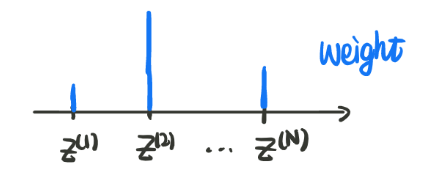
\includegraphics[width=.5\textwidth]{pic/微信图片_20191230154011.png}
    \caption{Sampling Importance Resampling示意图}
    \label{fig:my_label_1}
\end{figure}

通过二次采样可以降低采样不平衡的问题。至于为什么呢?大家想一想,我在这里表达一下自己的看法。$\frac{p(z_i)}{q(z_i)}$是Weight,如果Weight比较大的话,说明$p(z_i)$比较大而$q(z_i)$比较的小,也就是我们通过$q(z_i)$采出来的数量比较少。那么我们按权重再来采一次,就可以增加采到重要性样本的概率,成功的弥补了重要性采样带来的缺陷,有效的弥补采样不均衡的问题。

那么,权值大的样本我们就采样的比较多,权值小的样本就采样的比较少。这样就去掉了权值,换了一种方法等价的来表示重要程度。就可以解决权值退化的问题。

\subsection{How to do it?}
具体实现的思路其实就很简单。那就是根据概率密度函数(pdf)来计算得到概率分布函数(cdf)。然后通过从[0,1]之间进行均匀采样,来得到相应的的值。这个,我们在Markov Chain Monte Carlo 01 Sampling Method的\textbf{概率分布采样}中已经做了详细的描述。

讲到这里,Sampling Importance Resampling (SIR)实际上就是一种Basis Particle Filter,也就是SIS+Resampling,这是一种基本可以work的算法。

\subsection{找一个更好的$Q(Z)$}
选择$Q(z_t|z_{1:t-1},x_{1:t})=P(z_t|z_{t-1}^{(i)})$,用状态转移矩阵来进行定义,那么我们就可以将权值改写成:
\begin{equation}
    w_t^{(i)}  \propto  \frac{P(x_t|z_t^{(i)})P(z_t^{(i)}|z_{t-1})}{P(z_t|z_{t-1}^{(i)})} \cdot w^{(i)}_{t-1} = P(x_t|z_t^{(i)})\cdot w^{(i)}_{t-1}
\end{equation}
所以,$w_t^{(i)} = P(x_t|z_t^{(i)})\cdot w^{(i)}_{t-1}$,且$z^{(i)}\sim P(z_t|z_{t-1}^{(i)})$。改写后的算法为SIR Filter,也就是下列三个部分组成的:
\begin{center}
    Sequential Importance Sampling + Resampling + $Q(z_t|z_{1:t-1},x_{1:t})=P(z_t|z_{t-1}^{(i)})$
\end{center}
那么我们为什么要令$Q(z_t|z_{1:t-1},x_{1:t})=P(z_t|z_{t-1}^{(i)})$呢?因为在$t$时刻采样的时候,不是要去找一个新的分布,而是就从之前就用的一个中进行寻找。我们可以用一个很简单的例子来说明:就像很多人寻找自己的另一半,找了很久都没有合适的,直到最后才发现另一半就在自己身边的朋友中,也就是“兔子就吃窝边草”吧。我们用之前就算好的会方便很多。

我们用,{\color{red} generate and test},来描述这个过程非常的形象。Generate是$z_t\longrightarrow P(z_t|Z_{t-1}^{(i)})$,也就是状态转移矩阵。而Test是$w_{t-1}$,也就是$P(x_t|z_t^{(i)})$这个实际上就是发射矩阵,这个实际上是一举两得的作用。$P(x_t|z_t^{(i)})$越大一方面表示了发射矩阵的概率大;另一方面是表示了采样的权重很大,采出来的样本越重要,采样的效率越高。所以,$Q(z_t|z_{1:t-1},x_{1:t})=P(z_t|z_{t-1}^{(i)})$呢?因为在$t$起到了一语双关的重用,实现了共同目标的优化。

\section{Sampling Importance Resampling (SIR)总结}
\textbf{Sampling Importance Resampling Algorithm:}

前提:$t-1$时刻的采样都已经完成;

1.Sampling:

$t$时刻对于$N$个采样值,for i=1, 2,$\cdots$, N:
\begin{equation}
    z_t^{(i)}\sim P(z_t|z_{t-1}^{(i)})
\end{equation}
\begin{equation}
    w_t^{(i)}  \propto  \frac{P(x_t|z_t^{(i)})P(z_t^{(i)}|z_{t-1})}{P(z_t|z_{t-1}^{(i)})} \cdot w^{(i)}_{t-1} =P(x_t|z_t^{(i)})\cdot w^{(i)}_{t-1}
\end{equation}

end

2. Normalized:
\begin{equation}
    w_t^{(i)}\longrightarrow \hat{w}_t^{(i)},\quad \sum_{i=1}^N \hat{w}_t^{(i)} =1
\end{equation}


3. Resampling:
\begin{equation}
    \hat{\hat{w}}_t^{(i)} = \frac{1}{N}
\end{equation}
\end{document}
